\documentclass[11pt,a4paper]{article}
\usepackage[margin=2.0cm]{geometry}
\usepackage{graphicx}
\usepackage{booktabs}
\usepackage{amsmath}
\usepackage{hyperref}
\usepackage{xcolor}
\usepackage{float}
\usepackage{caption}
\usepackage{enumitem}
\usepackage{multicol}

\hypersetup{colorlinks=true, linkcolor=blue!60!black, urlcolor=blue!60!black}
\setlength{\parskip}{0.4em}
\setlength{\parindent}{0pt}

\title{\textbf{Solar Farm DA Bid Strategy}\\[0.3em]
\large 1~MW East-West --- Slovak Market, Spring-Summer}
\author{Quantitative Analysis}
\date{March 2026}

\begin{document}
\maketitle
\vspace{-1.5em}

\section*{The Question}

A 1~MW solar farm (half east, half west facing, 35\textdegree{} tilt, Bratislava) produces approximately 684~MWh over March--August. Each hour we choose: \textbf{sell on DA} at a minimum bid price, or \textbf{skip DA} and settle at the imbalance price. When skipping DA, we can \textbf{curtail} production during hours when a volume predictor flags large system surplus. The predictor gives us predicted imbalance volume (MWh), not price. What DA bid threshold maximises revenue?

\section*{The Strategy}

\begin{enumerate}[leftmargin=*, itemsep=0.1em]
    \item \textbf{DA price $\geq$ bid threshold} $\rightarrow$ Sell on DA (committed delivery).
    \item \textbf{DA price $<$ threshold, predictor says large surplus} $\rightarrow$ Curtail (avoid negative prices).
    \item \textbf{DA price $<$ threshold, predictor says deficit/small surplus} $\rightarrow$ Produce at imbalance price.
\end{enumerate}

\textbf{Curtailment budget:} rank the hours that didn't sell on DA by predicted surplus volume (largest \texttt{imbalance\_mwh} first). Curtail up to 50\% of that volume, allocated to the biggest surplus hours. The 50\% refers to MWh of production, not number of hours.

\section*{Key Result}

\begin{table}[H]
\centering
\begin{tabular}{lrrr}
\toprule
\textbf{Strategy} & \textbf{Opt. Bid} & \textbf{EUR/MWh} & \textbf{Season Total} \\
\midrule
\textbf{Hybrid (curtail top 50\%)} & \textbf{58 EUR} & \textbf{62.2} & \textbf{42,581 EUR} \\
DA or nothing (curtail 100\%) & 0 EUR & 53.1 & 36,369 EUR \\
Pure DA (bid = 0) & 0 EUR & 50.8 & 34,762 EUR \\
\bottomrule
\end{tabular}
\end{table}

The hybrid strategy earns \textbf{+22.5\%} vs pure DA (+11.4~EUR/MWh) over 2025 spring-summer. Below 58~EUR, the imbalance market plus curtailment wins because the predictor dodges the worst surplus hours. Above 58~EUR, DA certainty wins because high DA prices ($>$112~EUR/MWh average) systematically beat imbalance.

\begin{figure}[H]
    \centering
    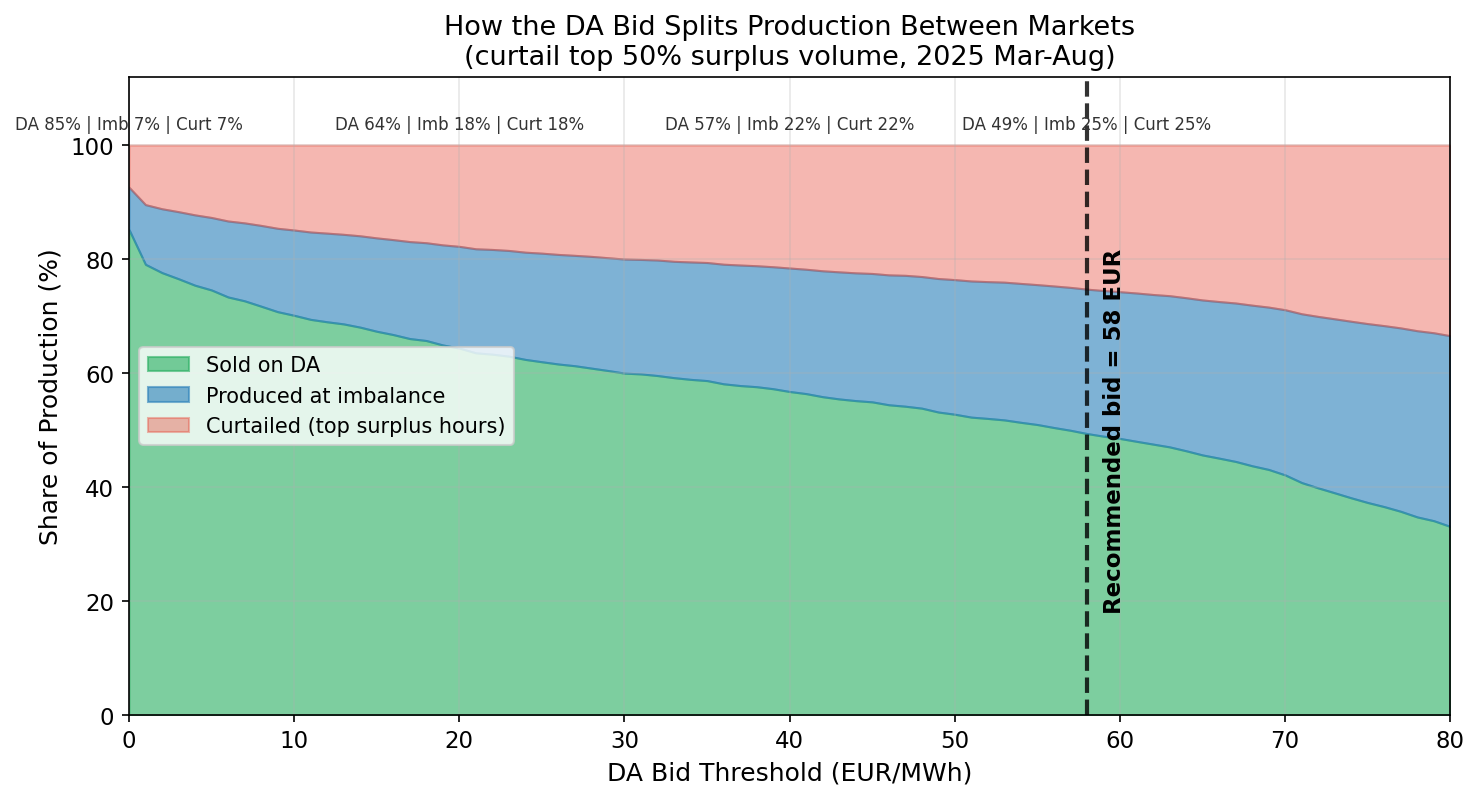
\includegraphics[width=0.85\textwidth]{07_bid_effect_zoomed.png}
    \caption{How the DA bid splits production between markets (0--80~EUR range). At bid~=~0, nearly everything goes to DA. As the bid rises, more hours are routed to imbalance or curtailed. At the recommended 58~EUR, roughly half the production sells on DA, a quarter produces at imbalance, and a quarter is curtailed during the worst surplus hours.}
\end{figure}

\begin{figure}[H]
    \centering
    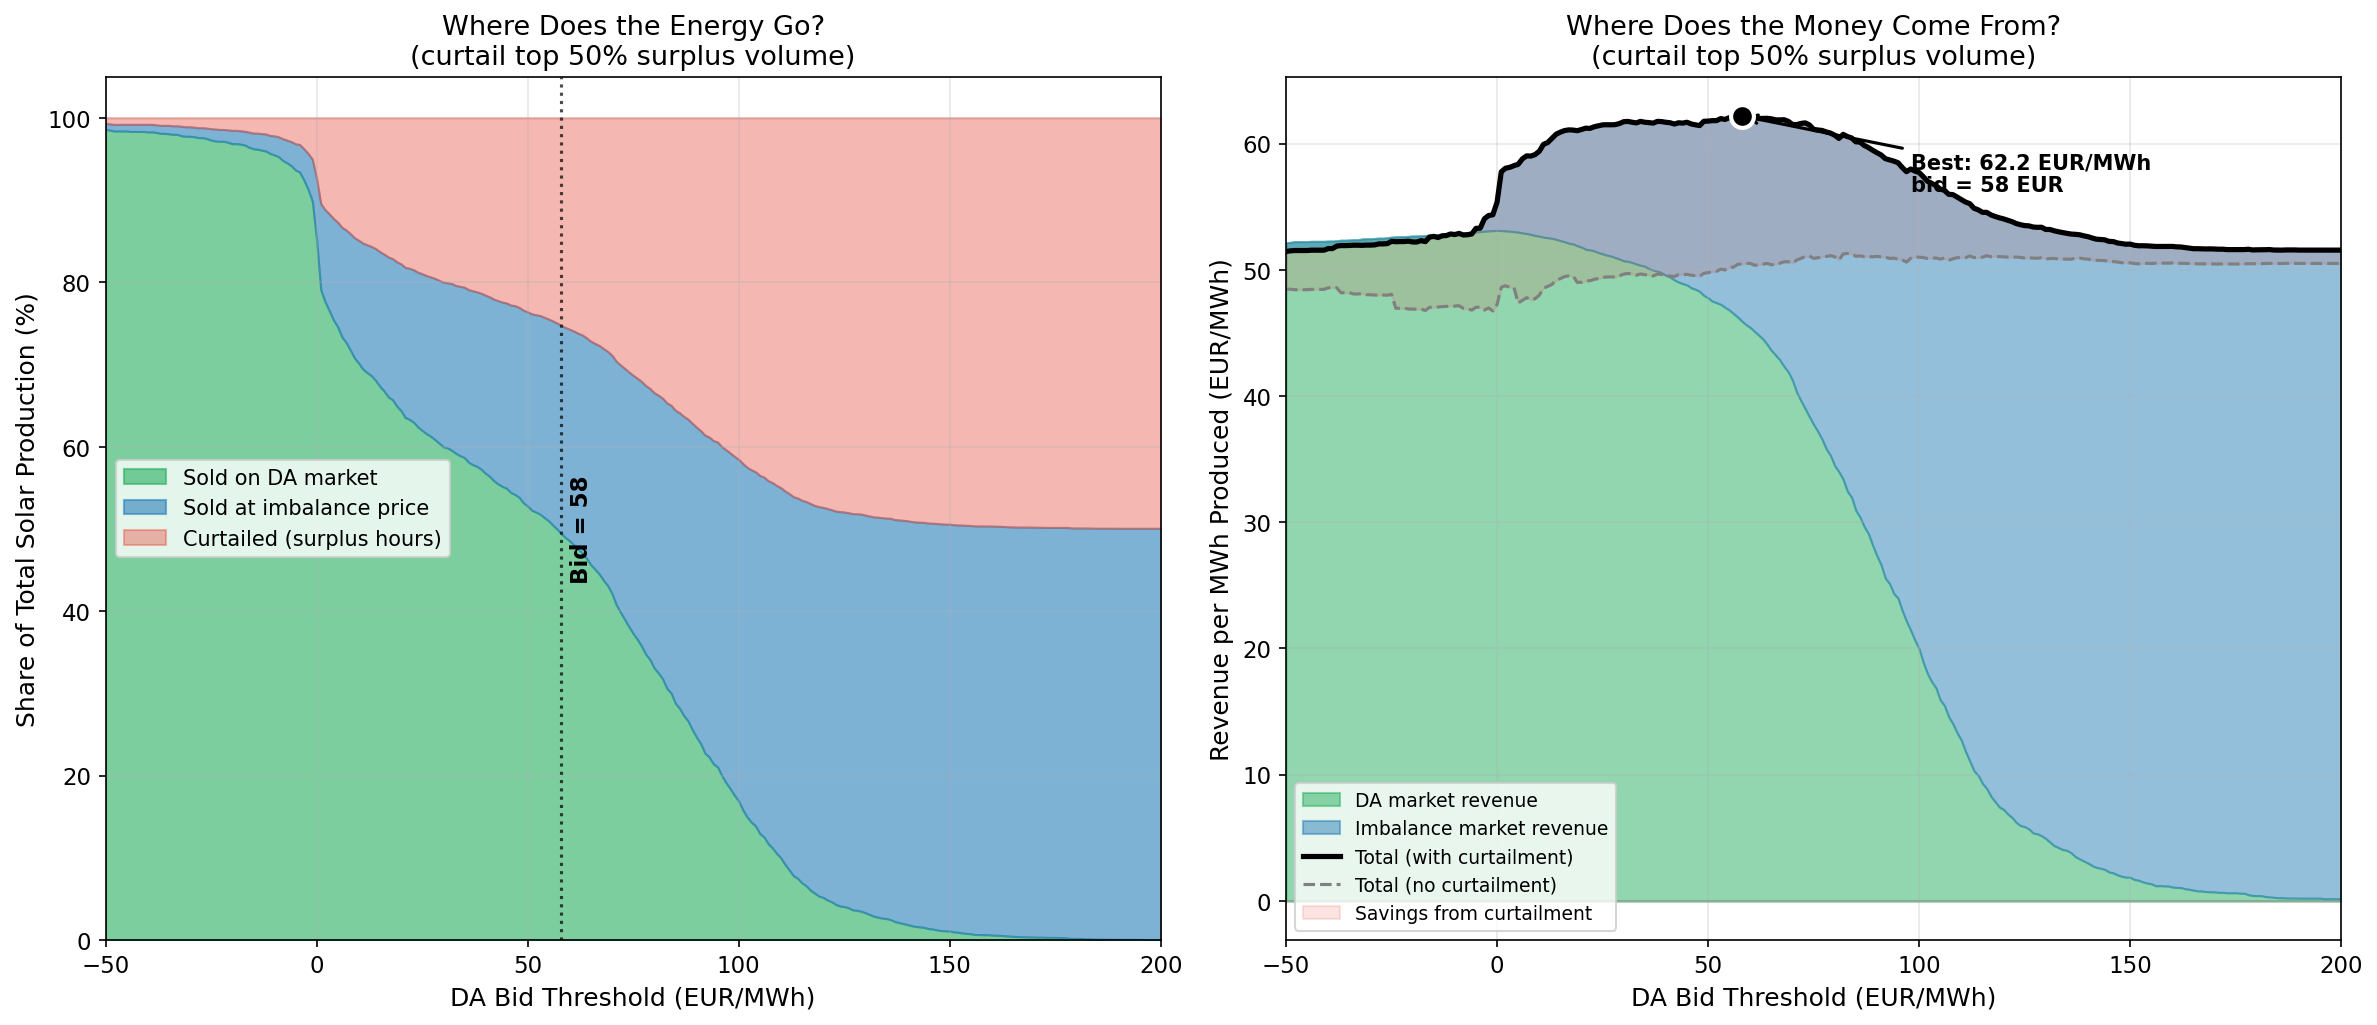
\includegraphics[width=0.85\textwidth]{01_revenue_composition.png}
    \caption{Left: share of production by market across the full bid range. Right: revenue per MWh by source. Solid line includes curtailment savings; dashed line shows revenue without curtailment. Peak at bid~=~58~EUR.}
\end{figure}

\newpage

\section*{Why 50\% Curtailment?}

The volume predictor is a noisy proxy for price---it ranks hours by surplus volume, not by how negative the price will be. The first 10\% of curtailment captures most of the value (51.3~$\rightarrow$~60.9~EUR/MWh). Going to 50\% squeezes out the rest (60.9~$\rightarrow$~62.2). Beyond 50\%, we start curtailing hours that actually had acceptable prices, so revenue drops. A perfect price oracle would earn $\sim$3,000~EUR/MW/season more.

\begin{figure}[H]
    \centering
    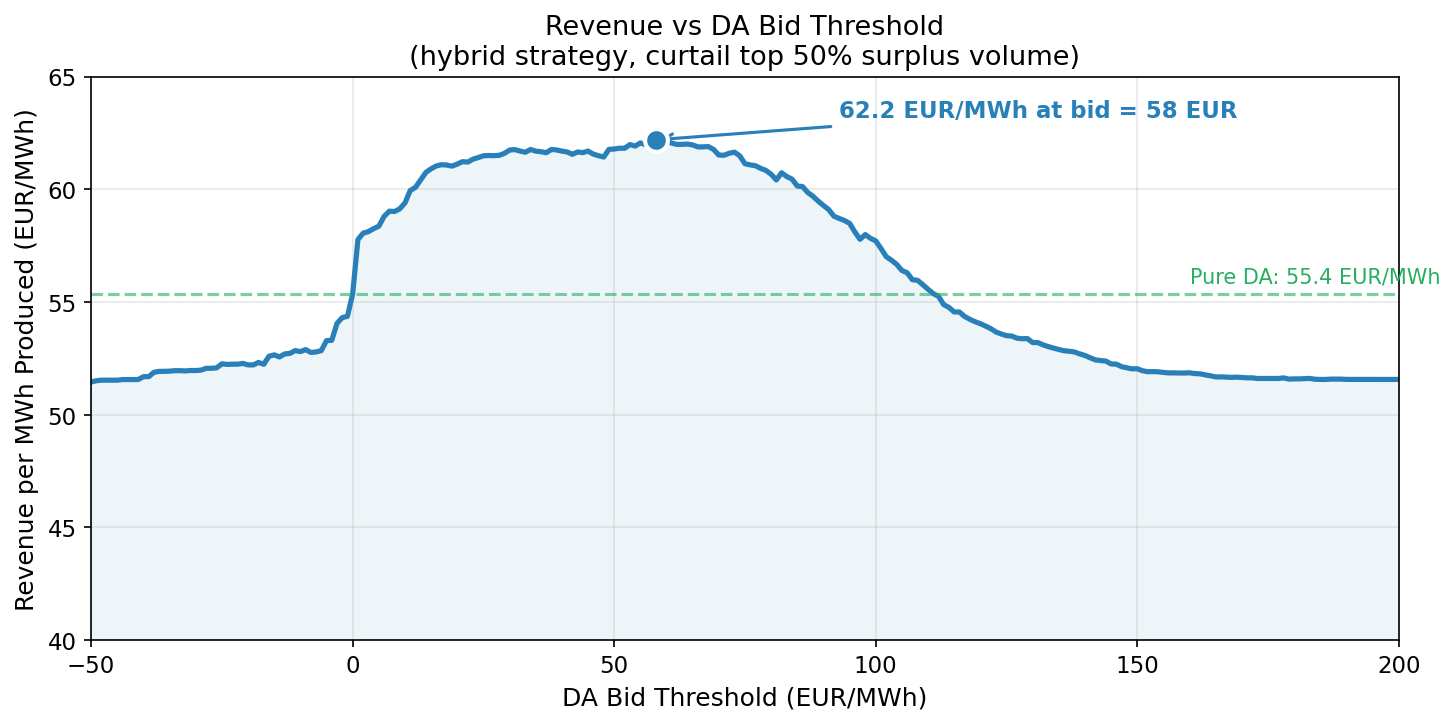
\includegraphics[width=0.85\textwidth]{07_revenue_vs_bid.png}
    \caption{Revenue per MWh vs DA bid threshold for the recommended strategy (curtail top 50\% surplus volume). Peak at 62.2~EUR/MWh, bid~=~58~EUR. Dashed line shows the pure DA baseline (50.8~EUR/MWh). The curve is flat near the peak, so bids in the 40--70~EUR range all perform well.}
\end{figure}

\section*{Seasonal Rules}

\begin{table}[H]
\centering
\begin{tabular}{llll}
\toprule
\textbf{Season} & \textbf{Months} & \textbf{DA Bid} & \textbf{Rationale} \\
\midrule
Winter & Nov--Feb & 0 EUR (pure DA) & DA beats imbalance, no surplus risk \\
Transition & Mar--Apr & 40--55 EUR & Few surplus events, small hybrid gain \\
Peak solar & May--Jun & 45--58 EUR & Surplus events spike, hybrid adds 10--15 EUR/MWh \\
Late summer & Jul--Aug & 40--55 EUR & Shorter days, moderate surplus \\
\bottomrule
\end{tabular}
\end{table}

2026 Feb--Mar confirms the winter rule: DA dominates at 96.3~EUR/MWh with no benefit from curtailment.

\section*{Solar Profile}

The plant is PVGIS-calibrated (v5.3): 0.5~MW East + 0.5~MW West, 35\textdegree{} tilt, 14\% system losses. Annual production: 943~MWh. The east-west split creates a double-peak pattern ($\sim$420~kW at 9--10h and 14--15h, dip to $\sim$385~kW at noon), which is advantageous: more production in morning/evening hours when prices are higher and system surplus is lower than at solar noon.

\section*{Practical Implications}

\begin{enumerate}[leftmargin=*, itemsep=0.1em]
    \item \textbf{March 2026 (now):} bid 40--55~EUR on DA. We are entering the transition period where curtailment starts to add value.
    \item \textbf{Predictor quality matters.} The volume predictor leaves $\sim$3,000~EUR/MW/season on the table vs a perfect price oracle. Incorporating wind/solar forecasts and cross-border flows could close this gap.
    \item \textbf{East-west beats south-facing} for this strategy: the flatter production profile avoids peak solar-surplus hours and earns more in the morning/evening price peaks.
\end{enumerate}

\end{document}
